% ---------------------------------------------------------------------------
%  Swiss Summer Student Particle Physics Program (S3P3) - Project Report
%  Compile (conda env "vulcanus"):  tectonic -X compile gmoretti_s3p3_report_v2.tex
% ---------------------------------------------------------------------------
\documentclass[10.5pt,a4paper]{article}

\usepackage{fontspec}
\setmainfont{Charter}
\setsansfont{Helvetica Neue}[UprightFont={Helvetica Neue},BoldFont={Helvetica Neue Bold},ItalicFont={Helvetica Neue Italic},BoldItalicFont={Helvetica Neue Bold Italic}]
\usepackage{unicode-math}
\setmathfont{STIX Two Math}

\usepackage[a4paper,top=2.5cm,bottom=2.2cm,left=2.1cm,right=2.1cm,
            headheight=40pt,headsep=12pt,footskip=26pt]{geometry}
\usepackage{graphicx,xcolor,enumitem,fancyhdr,titlesec,microtype,booktabs,array}
\usepackage[most]{tcolorbox}
\usepackage{tikz}
\usetikzlibrary{arrows.meta,positioning,calc,shapes.geometric,fit,backgrounds}
\usepackage{caption,subcaption}
\usepackage[hidelinks]{hyperref}

\graphicspath{{./}{../presentations/imgs/}{../presentations/S3P3_meeting/elements/}}

% --- Palette ---------------------------------------------------------------
\definecolor{s3p3blue}{RGB}{0,176,240}
\definecolor{navy}{RGB}{14,38,82}
\definecolor{ink}{RGB}{38,42,52}
\definecolor{mist}{RGB}{238,244,250}
\definecolor{okgreen}{RGB}{46,160,90}
\definecolor{warnorange}{RGB}{232,140,40}
\definecolor{rule}{RGB}{190,205,222}
\color{ink}

% --- Identity ----------------------------------------------------------------
\newcommand{\studentname}{Giacomo Moretti}
\newcommand{\supervisorname}{Marius K\"oppel}
\newcommand{\hostgroup}{Mu3e collaboration, SciFi detector group}
\newcommand{\hostinstitute}{D-PHYS, ETH Z\"urich}
\newcommand{\projecttitle}{Operating the Mu3e SciFi Detector}
\newcommand{\projectsub}{Control, Monitoring and Calibration}

% --- Header / footer ------------------------------------------------------
\pagestyle{fancy}
\fancyhf{}
\fancyhead[L]{\sffamily\footnotesize\color{navy}\textbf{Project Report} \textcolor{rule}{\textbar}\ July--September 2026}
\fancyhead[R]{
\includegraphics[height=0.95cm]{s3p3-logo.png}}
\fancyfoot[L]{\sffamily\footnotesize\textbf{\textcolor{s3p3blue}{2026 Swiss Summer Student Particle Physics Program}}\ \textcolor{rule}{\textbar}\ \studentname}
\fancyfoot[R]{\sffamily\footnotesize\textbf{\thepage}}
\renewcommand{\headrulewidth}{0.4pt}
\renewcommand{\headrule}{\color{rule}\hrule width\headwidth height 0.4pt}
\renewcommand{\footrulewidth}{0pt}
\fancypagestyle{plain}{\fancyhf{}\fancyfoot[R]{\sffamily\footnotesize\textbf{\thepage}}}

% --- Headings ----------------------------------------------------------------
\titleformat{\section}{\sffamily\Large\bfseries\color{navy}}
  {\textcolor{s3p3blue}{\thesection}}{0.55em}{}[\vspace{-0.55em}\textcolor{s3p3blue}{\rule{2.2cm}{1.4pt}}]
\titleformat{\subsection}{\sffamily\large\bfseries\color{navy}}
  {\textcolor{s3p3blue}{\thesubsection}}{0.55em}{}
\titlespacing*{\section}{0pt}{1.0em}{0.7em}
\titlespacing*{\subsection}{0pt}{0.9em}{0.35em}
\setlist[itemize]{leftmargin=1.2em,topsep=2pt,itemsep=2pt,label={\textcolor{s3p3blue}{\rule{3.6pt}{3.6pt}}}}
\setlength{\parskip}{0.42em}
\setlength{\parindent}{0pt}
\linespread{1.04}
\setcounter{secnumdepth}{2}

\newcommand{\pill}[1]{{\sffamily\bfseries\small\color{navy}#1}\;}
\captionsetup{font={small,sf},labelfont={bf,color=navy},labelsep=period,skip=4pt}

% --- Reusable boxes ------------------------------------------------------------
\newtcolorbox{callout}[1][]{enhanced,breakable,colback=mist,colframe=mist,
  borderline west={2.2pt}{0pt}{s3p3blue},boxrule=0pt,arc=1pt,
  left=8pt,right=8pt,top=5pt,bottom=5pt,#1}
\newcommand{\stat}[2]{\begin{tikzpicture}
  \node[draw=rule,rounded corners=2pt,fill=white,inner sep=5pt,minimum width=2.55cm,minimum height=1.25cm,align=center]
  {{\sffamily\bfseries\Large\color{navy}#1}\\[-1pt]{\sffamily\scriptsize\color{ink!80}#2}};
  \end{tikzpicture}}

\tikzset{
  blk/.style={draw=navy!70,fill=mist,rounded corners=2pt,align=center,font=\sffamily\scriptsize,
              inner sep=4pt,minimum height=0.85cm,text=ink},
  hub/.style={blk,fill=navy,draw=navy,text=white,font=\sffamily\scriptsize\bfseries},
  hot/.style={blk,fill=s3p3blue!15,draw=s3p3blue},
  arr/.style={-{Stealth[length=4pt]},draw=navy!80,line width=0.7pt},
  darr/.style={{Stealth[length=4pt]}-{Stealth[length=4pt]},draw=navy!80,line width=0.7pt},
  lab/.style={font=\sffamily\tiny,text=ink!80,inner sep=1.5pt,fill=white},
}

\begin{document}

% ============================ Title banner ===================================
\thispagestyle{plain}
\begin{tikzpicture}[remember picture,overlay]
  \fill[navy] (current page.north west) rectangle ([yshift=-5.0cm]current page.north east);
  \fill[s3p3blue] ([yshift=-5.0cm]current page.north west) rectangle ([yshift=-5.12cm]current page.north east);
  \node[anchor=north east,inner sep=0] at ([xshift=-2.1cm,yshift=-0.7cm]current page.north east)
       {
\includegraphics[height=1.7cm]{s3p3-logo.png}};
  \node[anchor=north west,inner sep=0,text width=13.4cm,font=\sffamily,text=white]
       at ([xshift=2.1cm,yshift=-0.85cm]current page.north west)
  {{\scriptsize\bfseries\color{s3p3blue!60!white}\MakeUppercase{Swiss Summer Student Particle Physics Program}}\\[1pt]
   {\scriptsize\color{white!70!navy}Project Report \textbullet\ July--September 2026}\\[10pt]
   {\fontsize{23}{26}\selectfont\bfseries \projecttitle}\\[3pt]
   {\Large\color{white!85!navy}\projectsub}\\[9pt]
   {\small\textbf{\studentname}\ \ \textcolor{s3p3blue}{\textbar}\ \ Supervisor: \supervisorname}\\[1pt]
   {\footnotesize\color{white!80!navy}\hostgroup, \hostinstitute}};
\end{tikzpicture}
\vspace*{2.5cm}

% ================================ Summary ====================================
\section*{\sffamily\Large\bfseries\color{navy}Summary}
\vspace{-0.3em}

The Mu3e experiment at the Paul Scherrer Institute (PSI) searches for the
charged-lepton-flavour-violating decay $\mu^+\to e^+e^-e^+$. In the Standard
Model it proceeds only through a neutrino loop, with a branching ratio of order
$10^{-54}$: it is effectively background-free, so any observation would be
unambiguous evidence of new physics. The current limit, $\mathcal{B}<10^{-12}$
(SINDRUM, 1988), leaves four orders of magnitude to explore, down to a
single-event sensitivity of about $10^{-16}$. This requires a continuous
$10^{8}\,\mu/\mathrm{s}$ beam and the suppression of two backgrounds: internal
conversion $\mu\to eee\nu\bar\nu$, controlled by momentum resolution, and
accidental combinatorics, controlled by timing and vertex resolution. The
scintillating-fibre (SciFi) detector provides the timing of the central region,
with a target resolution below $200\,\mathrm{ps}$.

\medskip
\begin{center}
\stat{2 rings}{12 modules each}\hspace{0.35em}%
\stat{96}{MuTRiG ASICs}\hspace{0.35em}%
\stat{3072}{readout channels}\hspace{0.35em}%
\stat{12}{front-end boards}\hspace{0.35em}%
\stat{24}{HV channels}
\end{center}

\pill{Project.} My project was the SciFi detector's control, monitoring and
calibration system, built end to end for the first physics run at PSI in October
2026. SciFi was operated through a single web page (\texttt{Scifi-monitor.js})
that had grown organically: it worked, but it was hard to trust and extend, and
it lagged behind the mature pixel-tracker tooling. I replaced it with a
structured set of Python control scripts that drive the hardware and a new
custom web page that a shift operator can rely on, both running inside the MIDAS
data-acquisition framework and communicating through its online database (ODB).

\pill{Method.} The system is built in layers: installation and bring-up at PSI;
the operator interface; the power chain (low voltage, high voltage, front-end
boards); a configuration and hardware-test hub; the two SiPM calibrations
(threshold and breakdown-voltage scans); and the saving of calibration results
to three destinations --- the live ODB, a local per-board cache and the
permanent calibration database (CDB).

\begin{callout}
\pill{Results.} The detector --- low voltage, high voltage, front-end boards and
readout --- is installed and working on the experiment back-end; the calibration
result-saving path is fully implemented and wired; and the shared
control-and-monitoring library now covers SciFi as well as the pixel detector.
The main item left is a full end-to-end test on the experiment, including a real
calibration run.

\pill{Personal contribution.} I designed and implemented the page, the
hardware-test hub, both calibrations and the saving path, and extended the
common library to SciFi. Alongside the software I took part in the on-site
detector work --- cabling, power distribution, assembly and repairs across the
full Mu3e detector --- and in the collaboration's weekly reports and meetings.
\end{callout}

\begin{center}
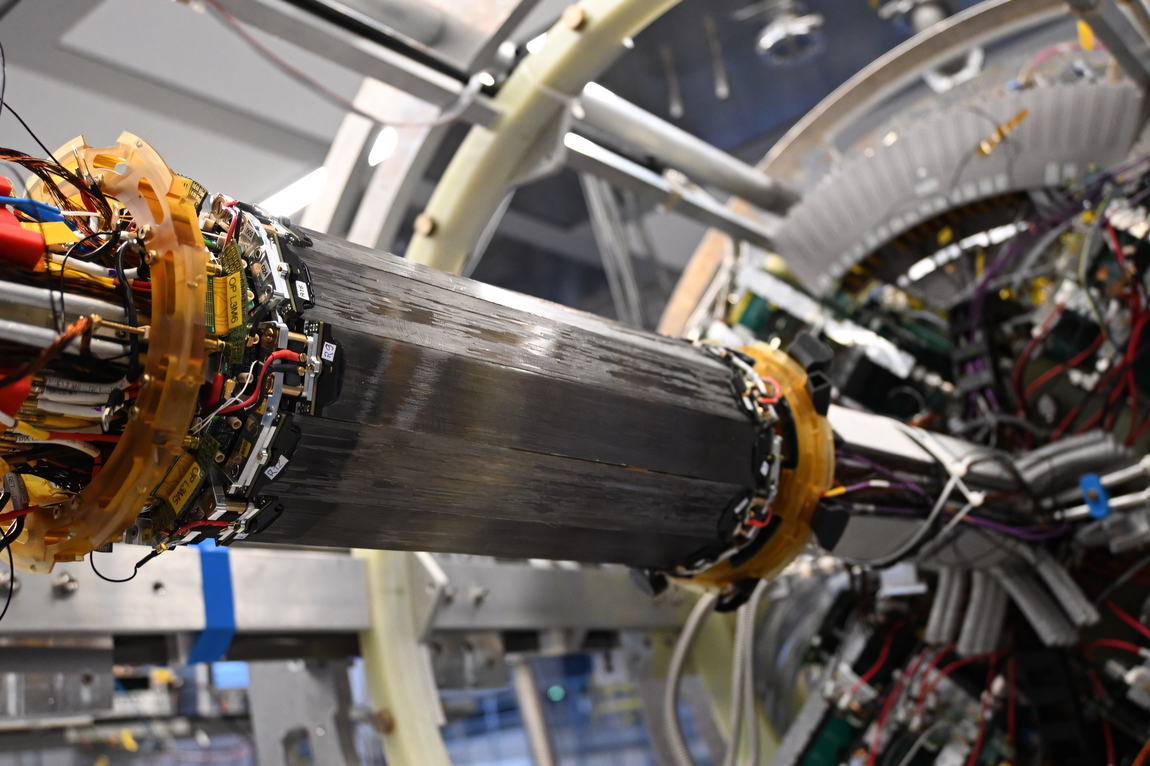
\includegraphics[width=0.8\linewidth,trim=0 200 0 200,clip]{img_install_wiring.png}
\captionof{figure}{The SciFi detector during installation at PSI.}
\end{center}

\clearpage

% ============================ Project details ================================
\section{Project Details}

\subsection{State of the art and objectives}

\pill{Physics context.}
Charged lepton flavour violation (cLFV) has never been observed. Neutrinos
oscillate, so lepton flavour is violated in the neutral sector, but for charged
leptons the Standard Model forbids it to any measurable level:
$\mu^+\to e^+e^-e^+$ needs a neutrino loop and is predicted at
$\mathcal{B}\sim10^{-54}$~\cite{tdr}. Many extensions of the Standard Model
raise this to within reach, making $\mu\to eee$ one of the ``golden'' muon
channels beside $\mu\to e\gamma$ and $\mu$--$e$ conversion. The strongest bound,
$\mathcal{B}<1.0\times10^{-12}$ (90\% C.L.), is from SINDRUM~\cite{sindrum};
Mu3e improves on it by four orders of magnitude using the most intense
continuous surface-muon beam in the world~\cite{tdr}.

\pill{Detector and DAQ.}
Mu3e reconstructs the three-electron final state with ultra-thin high-voltage
monolithic pixel sensors and measures time with two scintillator systems: the
SciFi detector in the central region ($<200\,\mathrm{ps}$) and scintillating
tiles in the recurl stations ($<50\,\mathrm{ps}$)~\cite{bravar,vigani}. SciFi
consists of an upstream (US) and a downstream (DS) ring of twelve modules each;
its 96 MuTRiG ASICs (32 channels each) are served by twelve front-end boards
and read out through the MIDAS framework~\cite{koppel}, whose online database
holds all configuration and slow-control data and whose web server hosts custom
operator pages. One module key --- side, ring position, readout end --- is used
consistently in the ODB, the geometry and the calibration~\cite{wang}.

\begin{figure}[ht]
\centering
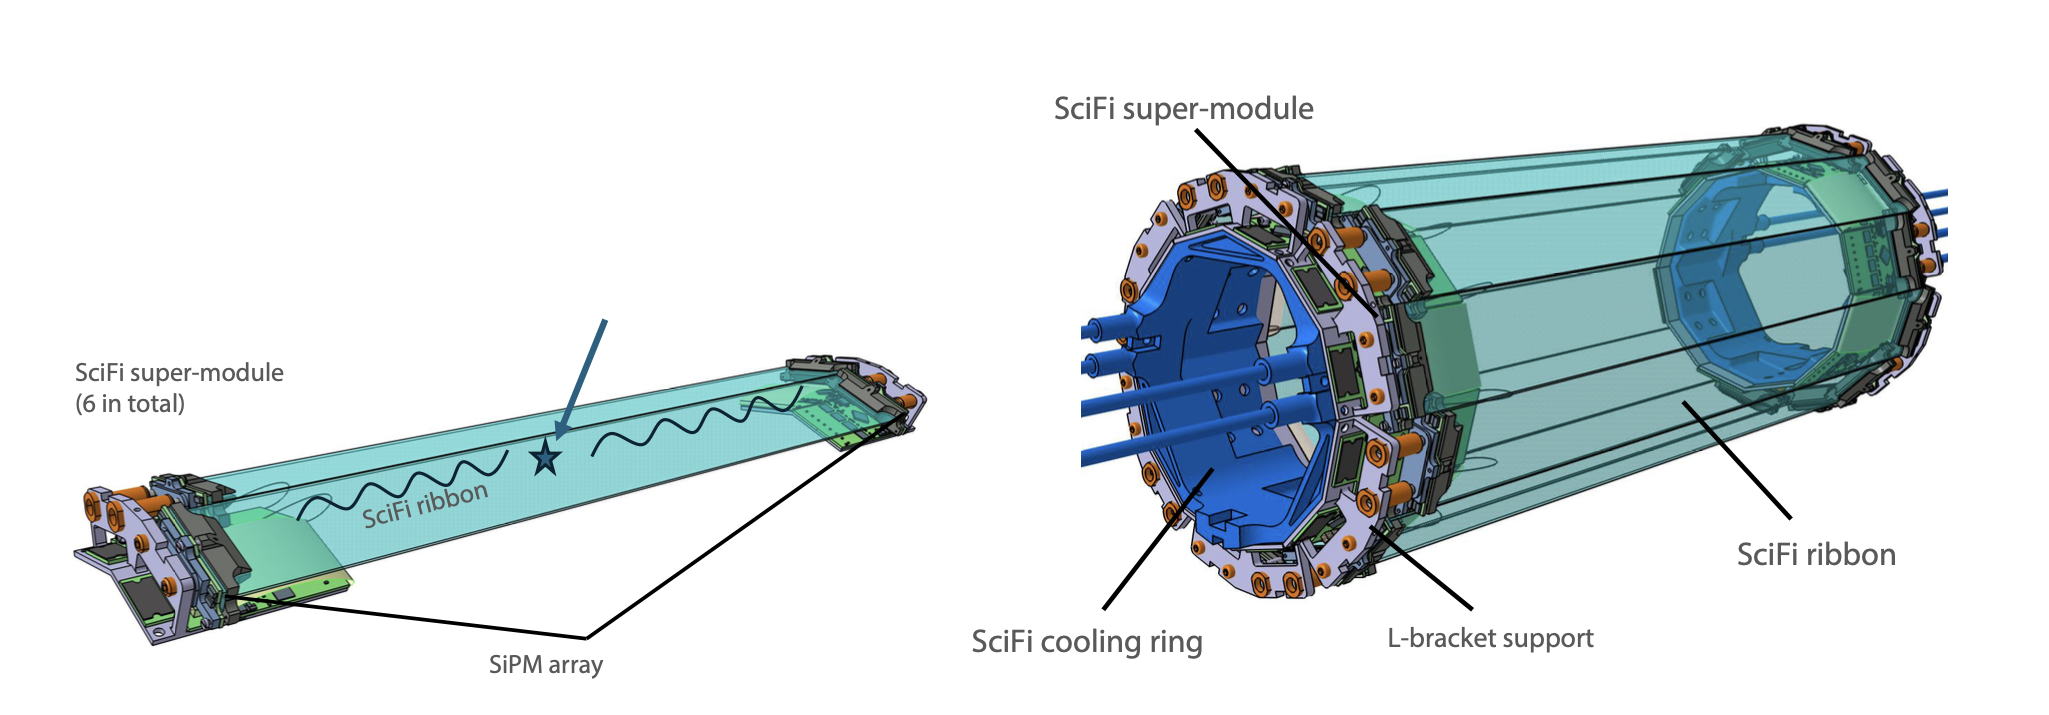
\includegraphics[width=0.93\linewidth]{scifi_render.png}
\caption{The SciFi detector: a fibre ribbon read out by SiPM arrays at both
ends (left) and the full cylinder with cooling rings and L-bracket supports
(right).}
\label{fig:scifi}
\end{figure}

\pill{Starting point.}
The pixel subdetector already had mature MIDAS integration: operator pages and
a structured library of Python control scripts. SciFi relied on one monitoring
page that had accreted features, with control logic spread over disconnected
scripts and no interface a shift operator could depend on during a run.

\pill{Objectives.}
With the first physics run in October 2026, SciFi needed
\textbf{(i)}~a coherent operator interface,
\textbf{(ii)}~a documented, reproducible calibration whose results reach the CDB,
and \textbf{(iii)}~a control code base shared with, rather than duplicating, the
pixel tooling. A dependable control system is a prerequisite for taking SciFi
data at all, and unified software lowers the long-term cost of running the
experiment.

\subsection{Methodology}

\pill{Environment.}
Everything targets the MIDAS DAQ: configuration and state live in the ODB,
operator interfaces are HTML/JavaScript pages served by MIDAS, and device logic
is Python on the front-end machine (Fig.~\ref{fig:arch}). No new physics data
was taken; the project builds on the ODB slow-control tree, the existing pixel
control library and the diverged SciFi scripts, and on the raw per-channel data
of the MuTRiG scans and hardware tests. The fixed hardware layout is the
reference against which ODB contents were checked. Development used a local
test ODB, then real hardware on the experiment back-end.

\begin{figure}[ht]
\centering
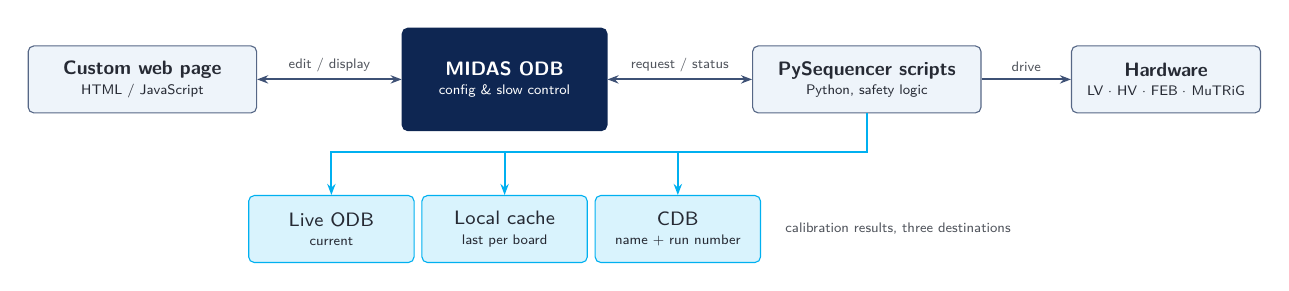
\begin{tikzpicture}[x=1cm,y=1cm]
  \node[blk,minimum width=2.9cm] (page) at (0,0) {\textbf{Custom web page}\\[-1pt]\tiny HTML / JavaScript};
  \node[hub,minimum width=2.6cm,minimum height=1.3cm] (odb) at (4.6,0) {MIDAS ODB\\[-1pt]\tiny\mdseries config \& slow control};
  \node[blk,minimum width=2.9cm] (py) at (9.2,0) {\textbf{PySequencer scripts}\\[-1pt]\tiny Python, safety logic};
  \node[blk,minimum width=2.4cm] (hw) at (13.0,0) {\textbf{Hardware}\\[-1pt]\tiny LV $\cdot$ HV $\cdot$ FEB $\cdot$ MuTRiG};
  \draw[darr] (page) -- node[lab,above=1pt]{edit / display} (odb);
  \draw[darr] (odb) -- node[lab,above=1pt]{request / status} (py);
  \draw[arr] (py) -- node[lab,above=1pt]{drive} (hw);
  \node[hot,minimum width=2.1cm] (live) at (2.4,-1.9) {Live ODB\\[-1pt]\tiny current};
  \node[hot,minimum width=2.1cm] (cache) at (4.6,-1.9) {Local cache\\[-1pt]\tiny last per board};
  \node[hot,minimum width=2.1cm] (cdb) at (6.8,-1.9) {CDB\\[-1pt]\tiny name + run number};
  \draw[arr,s3p3blue] (py.south) |- ($(cache.north)+(0,0.55)$) -| (live.north);
  \draw[arr,s3p3blue] ($(cache.north)+(0,0.55)$) -- (cache.north);
  \draw[arr,s3p3blue] ($(cache.north)+(0,0.55)$) -| (cdb.north);
  \node[lab,anchor=west] at ([xshift=0.25cm]cdb.east) {calibration results, three destinations};
\end{tikzpicture}
\caption{Architecture. All state flows through the ODB. The page never talks to
the hardware: it writes requests that a Python script executes, and calibration
results fan out to three destinations.}
\label{fig:arch}
\end{figure}

\pill{Existing vs.\ new.}
The pixel pages and scripts were the existing method and served as template:
the same web-server/ODB binding pattern and the same \emph{page-first}
workflow --- mock up the layout, agree the control granularity with the SciFi
experts, then write the Python backend. What had to be built was the entire
SciFi page and its ODB bindings (the pixel page does not fit the different
topology); SciFi coverage in the shared library, factored around
subdetector-agnostic abstractions for front-end board, ASIC and channel; a
configuration tab that doubles as the hardware-test hub; and two SiPM
calibrations on a common lifecycle with a working path to permanent storage.

\pill{Interface.}
A read-only \emph{Geometry} view --- a drill-down from super-module to module to
the 32-channel ASIC grid, drawn as mirrored US and DS rings --- sits beside the
editable \emph{Power}, \emph{Readout} and \emph{Calibration} tabs. Every
editable value goes to the ODB, from where a front-end process applies it.
Safety logic stays in Python and is never duplicated in JavaScript; no action is
ever hard-blocked --- the page warns rather than refuses.

\begin{figure}[t]
\centering
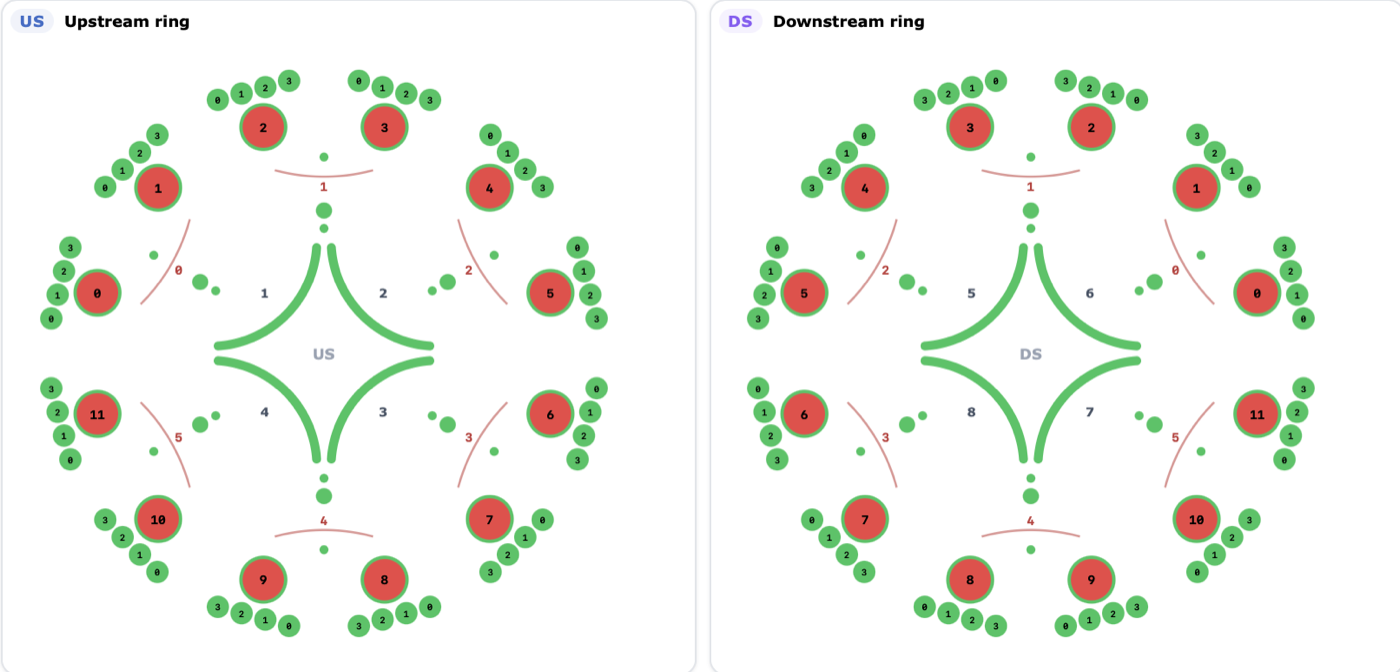
\includegraphics[width=0.55\linewidth]{img_page_new.png}\hfill
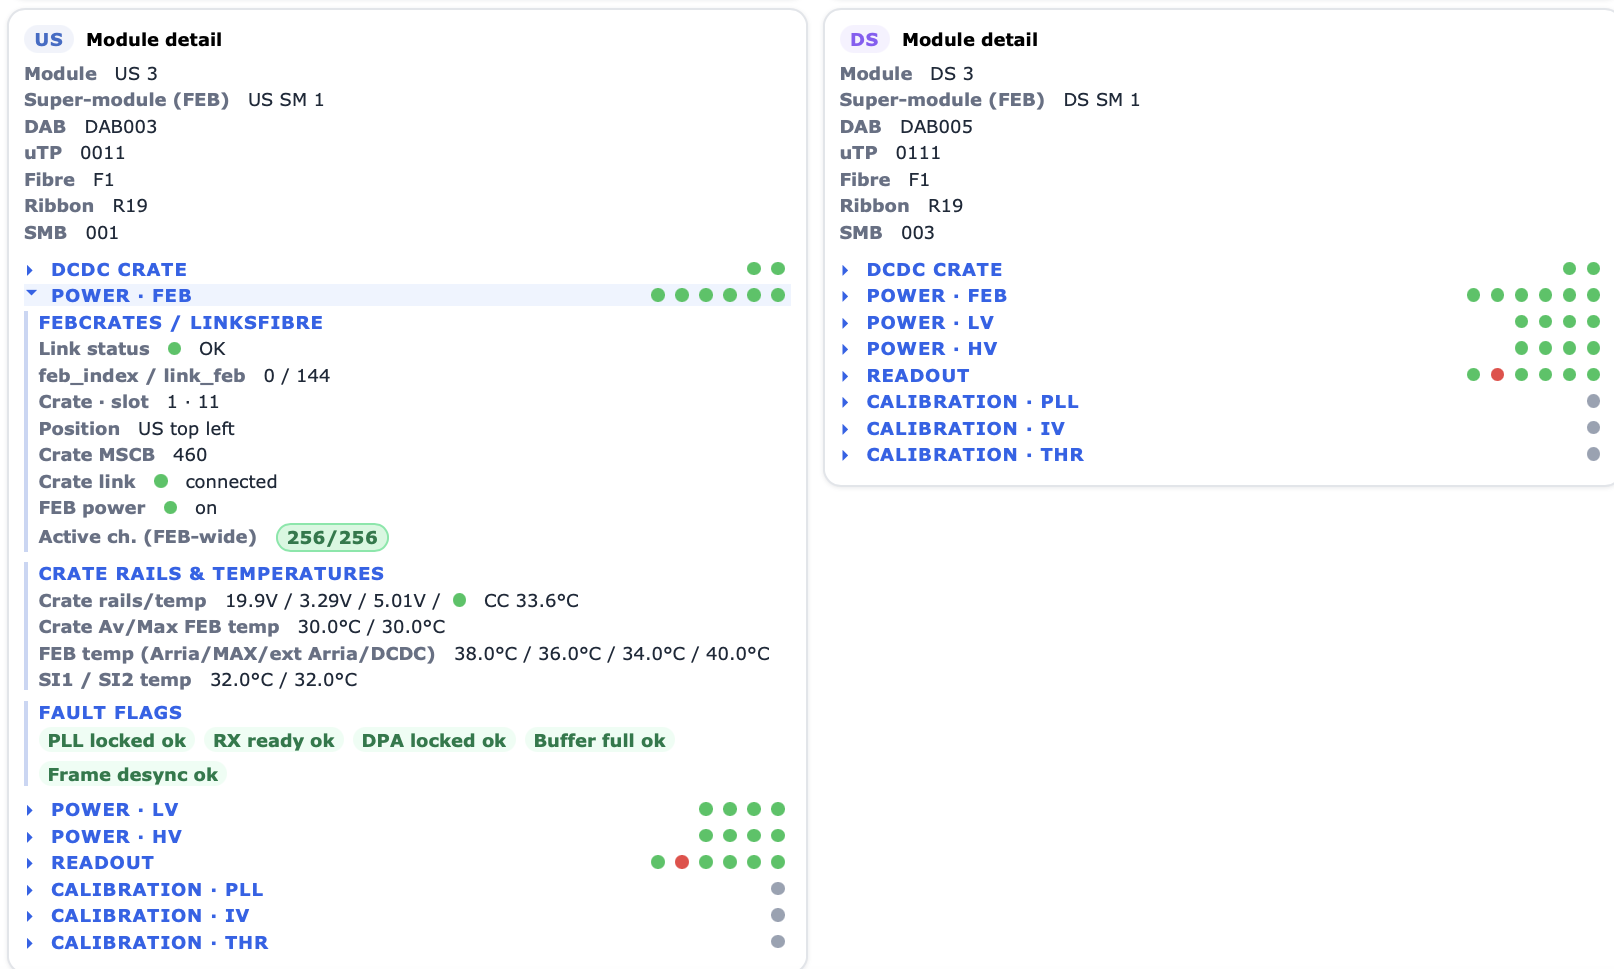
\includegraphics[width=0.42\linewidth]{img_geometry_drilldown.png}
\caption{The geometry view of the new operator page. Left: live US and DS rings,
with per-module, per-ASIC and per-crate state encoded in colour. Right:
drill-down into one module, with collapsible Power, Readout and Calibration
sections and fault flags.}
\label{fig:page}
\end{figure}

\pill{Configuration and hardware tests.}
The configuration tab walks the front-end board $\to$ module $\to$ chip
$\to$ channel tree, writes to a dedicated ODB subtree, and runs three tests:
\textbf{PLL} (each board must recover the clock from its data link --- the
recovered-clock delay histogram is flat when locked and sharply peaked when
not), \textbf{PRBS} (link integrity) and \textbf{TDC} (per-channel test pulse).

\pill{Calibration.}
Two per-board scans share one \texttt{prepare\,/\,execute\,/\,finalise}
lifecycle. The \emph{threshold scan} walks the discriminator threshold on each
channel and reads the rate curve to find the 0.5, 1.5 and 2.5 photo-electron
crossings; the result is loaded as operating threshold. The
\emph{breakdown-voltage scan} differentiates each SiPM's current--voltage curve
and fits a Gaussian to the peak, whose mean is the breakdown voltage and
therefore sets the operating overvoltage (Fig.~\ref{fig:vbr}). Each scan runs
independently per board, so any subset of the detector can be re-calibrated. A
run is requested from the page via the ODB; the PySequencer launches the
script, which opens its own MIDAS connection (explicitly closed on exit).

\begin{figure}[ht]
\centering
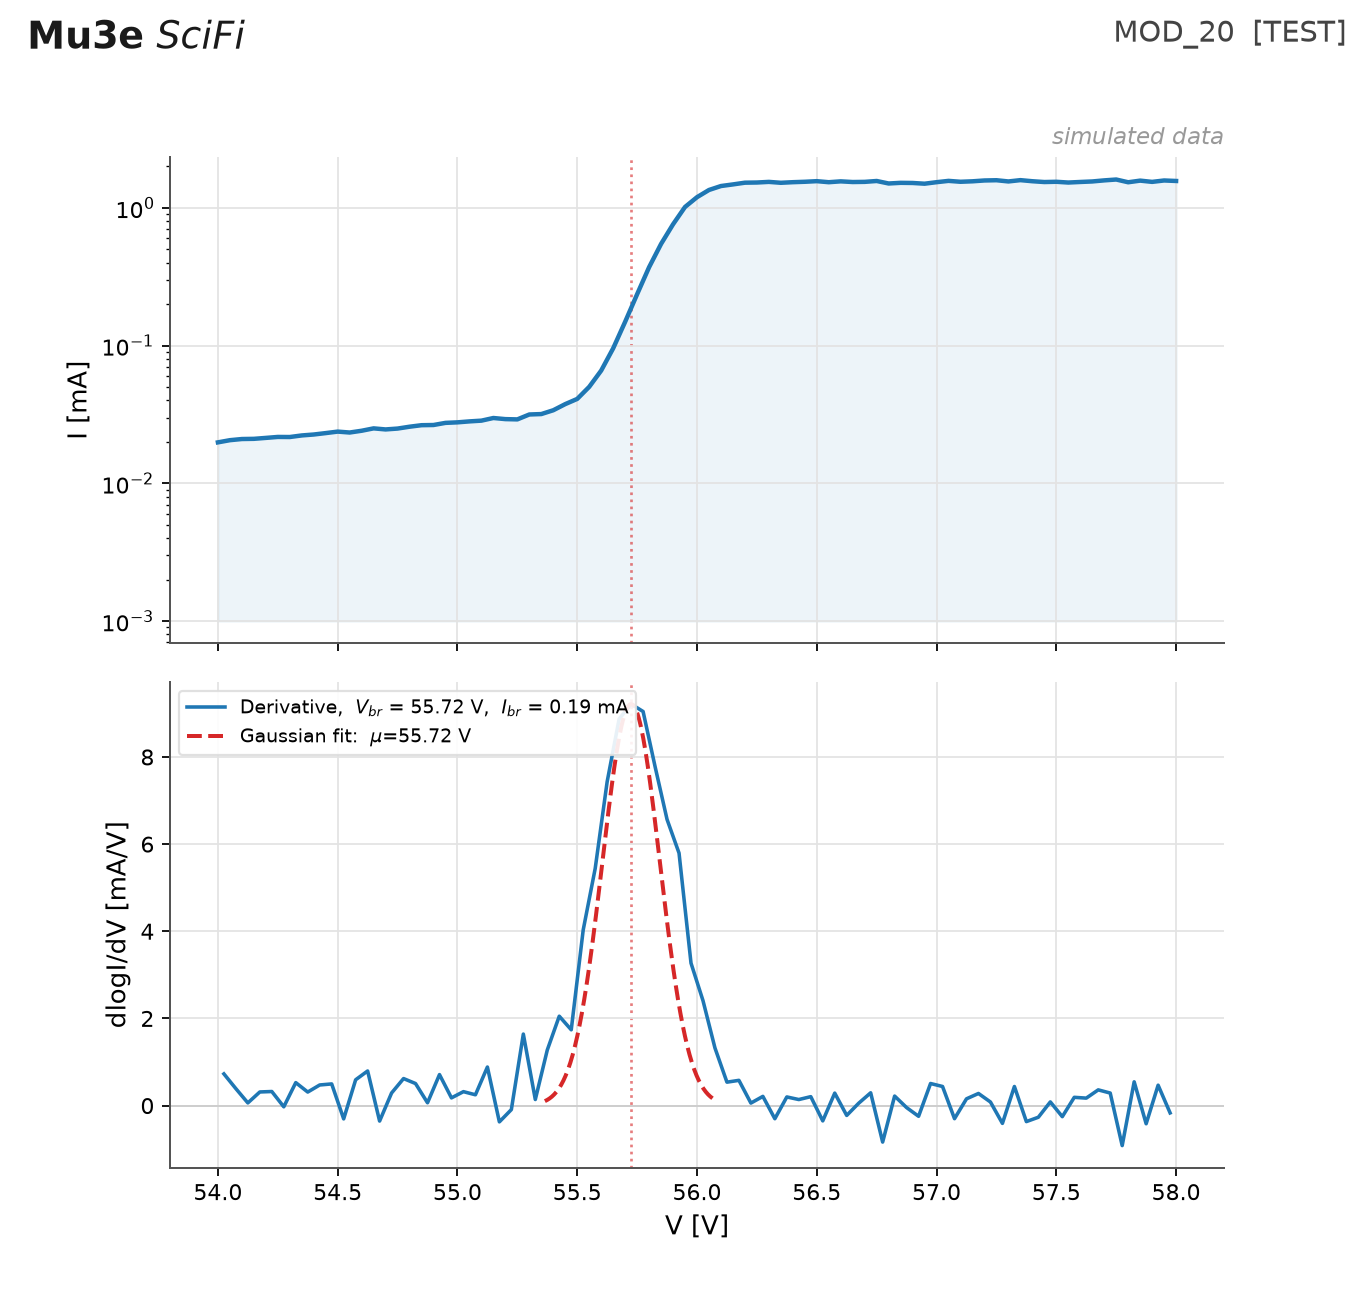
\includegraphics[height=6.4cm]{test_plot_vbr.png}\hfill
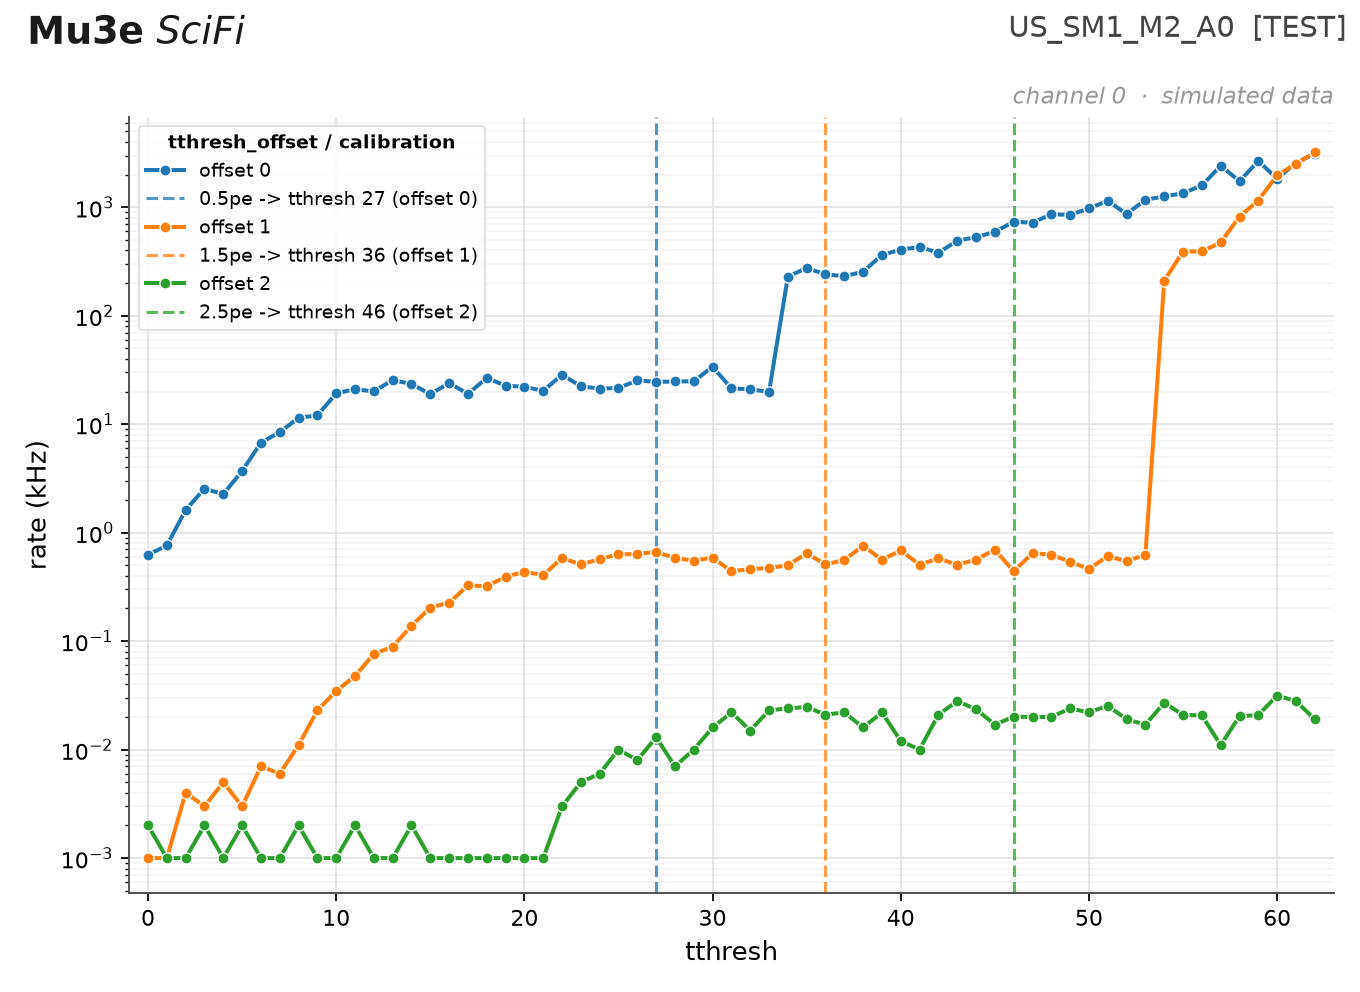
\includegraphics[height=6.4cm]{test_plot_thr.png}
\caption{Output of the two calibration scans on simulated data (test ODB). Left:
current--voltage curve and Gaussian fit to its derivative, giving the breakdown
voltage ($V_{br}=55.72$~V for this test module). Right: threshold scan.}
\label{fig:vbr}
\end{figure}

\pill{Saving.}
Each destination answers one question: the \textbf{live ODB} (\emph{what is the
calibration right now?}, overwritten each scan), the \textbf{local cache} of
the latest calibration per board (\emph{what did we last do, day to day?}) and
the permanent \textbf{CDB} indexed by name and run number (\emph{what was it on
a given run?}). The on-disk format is a small ROOT file with trees for
metadata, raw scan, results, conditions and channel masks. This path was
reconciled with a colleague's parallel work on the same code.

\pill{Verification and on-site work.}
Each branch --- power bring-up, hardware tests, calibration scans --- was built
and checked alone before merging, first on the local test ODB and then on real
hardware. The software grew inside the on-site campaigns at PSI, where I also
worked on cabling, power distribution, assembly and repairs; the power and
readout chains the page represents are largely those I helped bring up by hand.

\subsection{Results}

All three objectives were met and everything that had to be ready for the
October run is in place (Table~\ref{tab:res}).

\begin{table}[h]
\centering\small\sffamily
\renewcommand{\arraystretch}{1.25}
\begin{tabular}{@{}p{3.3cm}p{9.3cm}p{1.6cm}@{}}
\toprule
\textbf{Objective} & \textbf{Outcome} & \textbf{Status}\\
\midrule
Operator interface & New page replaces \texttt{Scifi-monitor.js}; Power, Readout,
Calibration bound to the ODB; Geometry view and readout-status monitoring
(rate, run state, buffers) integrated --- ``power all green'' and ``data
flowing'' shown as two distinct conditions & \textcolor{okgreen}{\textbf{done}}\\
Hardware tests & Configuration tab became the test hub, absorbing the Readout
tab; PLL, PRBS, TDC return one verdict per board or link & \textcolor{okgreen}{\textbf{done}}\\
Calibration \& saving & Both scans run per board and produce the loaded
threshold and overvoltage; saving to live ODB, local cache and CDB fully
implemented, ROOT layout finalised & \textcolor{okgreen}{\textbf{done}}\\
Shared code & Common library covers SciFi and pixel; duplication removed &
\textcolor{okgreen}{\textbf{done}}\\
Experiment status & LV, HV, FEBs and readout up; operated through the new page
during installation week at PSI & \textcolor{okgreen}{\textbf{done}}\\
End-to-end test & Page $\to$ real calibration run $\to$ all three destinations &
\textcolor{warnorange}{\textbf{open}}\\
\bottomrule
\end{tabular}
\caption{Results against the planned objectives.}
\label{tab:res}
\end{table}

\pill{Expectations and outlook.}
The delivered scope matches what was agreed with the SciFi group; the one
deviation --- the configuration tab growing into a full test hub --- was in the
useful direction. The principal open item is a single end-to-end test on the
experiment with a real calibration run. Smaller follow-ups: move the hardcoded
32-cell HV board-to-module map into Python/ODB, extend the online monitoring
histograms, and wire SciFi's own \texttt{CalibrationFactory} to a real entry
point so the scripts no longer need their direct-construction path.

\subsection{Contributions as an S3P3 student}

I worked within the \hostgroup{}, in coordination with the pixel DAQ developers,
who own the shared code and whose tooling was the reference. The system
described above is my own work:

\begin{itemize}
  \item the new custom page end to end --- Geometry view, Power / Readout /
  Calibration tabs, ODB bindings and Python backend --- and the design decisions
  behind it (safety logic in Python only; warn, never block);
  \item the configuration tab as hardware-test hub, with the PLL, PRBS and TDC flows;
  \item the threshold and breakdown-voltage calibrations on their shared
  lifecycle and the full saving path to ODB, cache and CDB, including the ROOT
  layout and its reconciliation with a colleague's branch;
  \item the extension of the common control library to SciFi.
\end{itemize}

\pill{Hardware, service and collaboration.}
Software was half the work. On site at PSI I did SciFi cabling and
power-distribution management, mechanical assembly and repairs, and designed
small hardware components; much of my time went to general service work across
the full Mu3e detector, including other subdetectors. I reported weekly, took
part in subdetector and DAQ meetings, and coordinated continuously with the DAQ
team, whose shared code the SciFi tooling extends rather than duplicates.

\begin{figure}[ht]
\centering
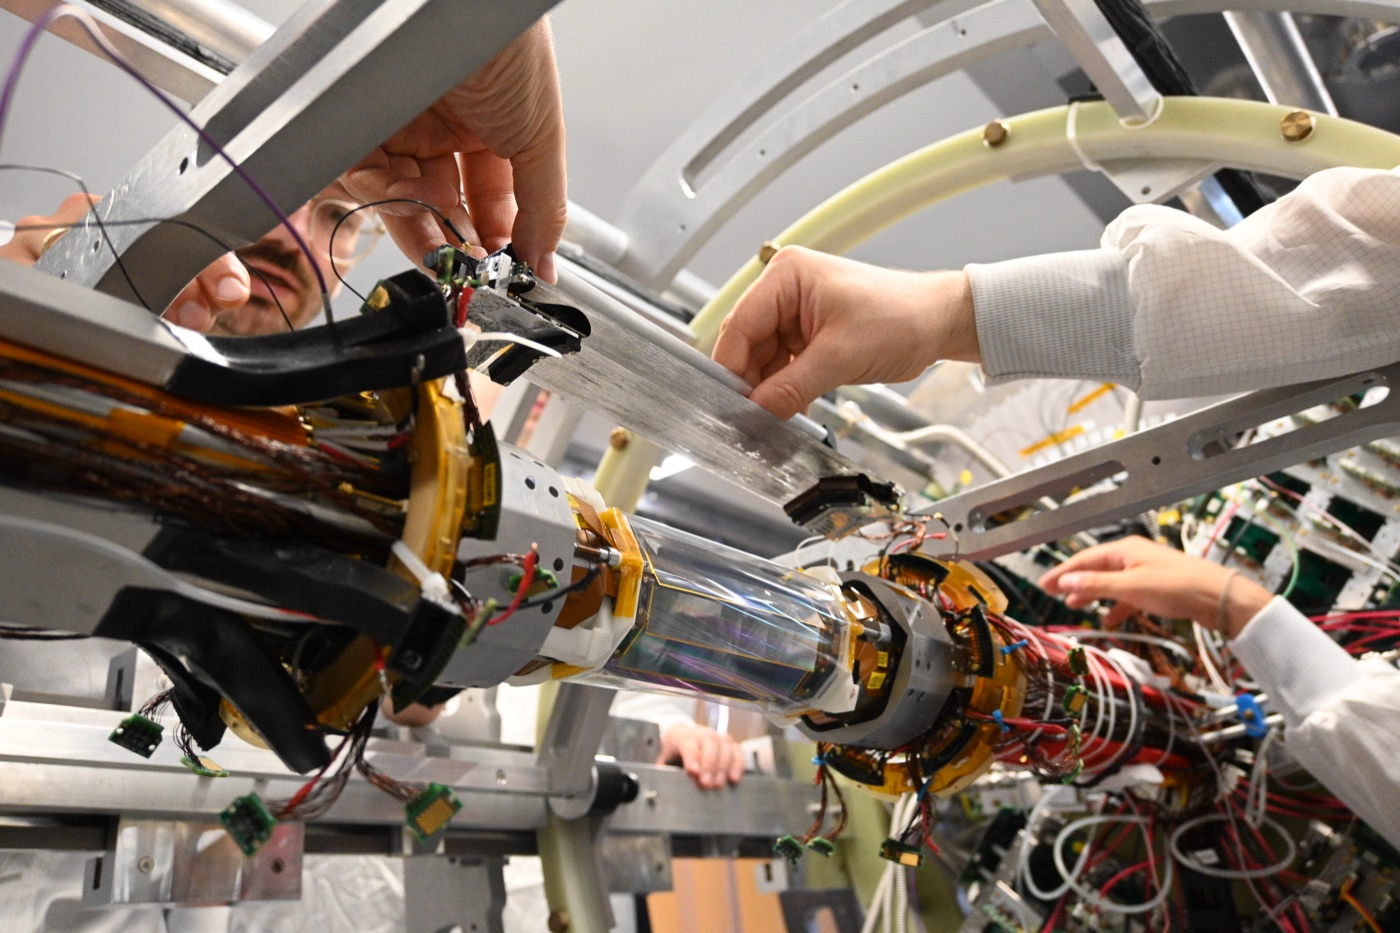
\includegraphics[width=0.485\linewidth]{img_install_assembly.jpg}\hfill
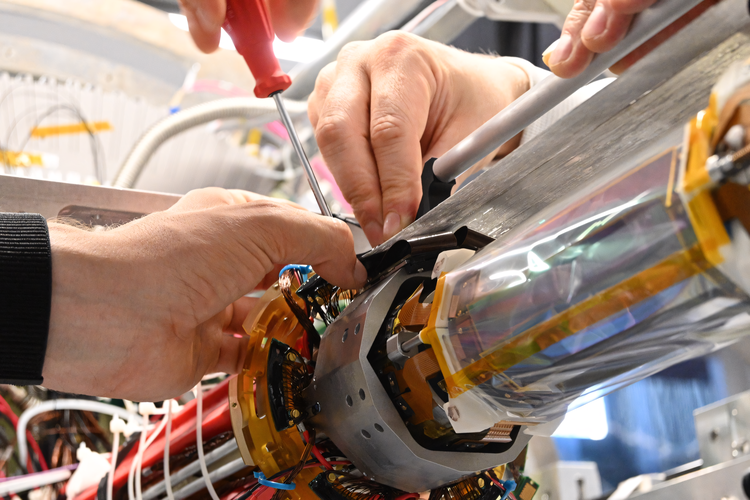
\includegraphics[width=0.485\linewidth]{img_install_detail.png}
\caption{On-site work at PSI: assembly and cabling of the detector.}
\end{figure}

% ================================ References =================================
\begin{thebibliography}{9}\small\sffamily
\bibitem{tdr} Mu3e Collaboration, ``Technical design of the Phase~I Mu3e experiment'', arXiv:2009.11690 (2021).
\bibitem{sindrum} U.~Bellgardt \textit{et al.} (SINDRUM Collaboration), ``Search for the decay $\mu^+\to e^+e^+e^-$'', Nucl.\ Phys.\ B \textbf{299} (1988) 1.
\bibitem{bravar} A.~Bravar \textit{et al.}, ``Development of the Scintillating Fibre Timing Detector for the Mu3e Experiment'', arXiv:2208.09906 (2022).
\bibitem{vigani} L.~Vigani \textit{et al.}, ``The Mu3e detector'', JINST \textbf{17} (2022) C05024.
\bibitem{koppel} M.~K\"oppel (Mu3e Collaboration), ``Mu3e Integration Run 2021'', arXiv:2203.07855 (2022).
\bibitem{wang} Y.~Wang (Mu3e Collaboration), ``The DAQ system of the Mu3e SciFi detector'', SPS/APS Joint Annual Meeting (2023).
\end{thebibliography}

\end{document}
